\documentclass[]{../resources/final_report}
\usepackage{graphicx}
\usepackage[hidelinks]{hyperref}
\usepackage{amsmath}
\usepackage{amssymb}
\usepackage[toc,page]{appendix}
\usepackage{wrapfig}
\graphicspath{{../resources/images/}}

\newcommand{\Reals}{\mathbb{R}}


%%%%%%%%%%%%%%%%%%%%%%
%%% Input project details
\def\studentname{Roger Milroy}
\def\reportyear{2019}
\def\projecttitle{Autonomous Micro Air Vehicles: Enhanced Navigation in GPS denied environments.}
\def\supervisorname{Professor Sara Bernadini}
\def\degree{BSc (Hons) in Computer Science (Artificial Intelligence)}
\def\fullOrHalfUnit{Full Unit} % indicate if you are doing the project as a Full Unit or Half Unit
\def\finalOrInterim{Interim Report} % indicate if this document is your Final Report or Interim Report

\begin{document}

\maketitle

%%%%%%%%%%%%%%%%%%%%%%
%%% Declaration

\chapter*{Declaration}

This report has been prepared on the basis of my own work. Where other published and unpublished source materials have been used, these have been acknowledged.

\vskip3em

Word Count: 11358

\vskip3em

Student Name: \studentname

\vskip3em

Date of Submission: March 20th 2020

\vskip3em

Signature: Roger Milroy

\newpage

%%%%%%%%%%%%%%%%%%%%%%
%%% Table of Contents
\tableofcontents\pdfbookmark[0]{Table of Contents}{toc}\newpage

%%%%%%%%%%%%%%%%%%%%%%
%%% Your Abstract here

\begin{abstract}

A core competence for cyber-physical systems is that of pose estimation. This is all the more 
important where there is any element of autonomy. Where automated systems can manoeuvre any 
physical body such as a car, plane or drone it needs to have a robust estimate of it’s position 
and preferably it’s position relative to other objects, without this it would be unable to manoeuvre effectively.

In the context of Micro Air Vehicles (MAVs) this task is more challenging due to weight and cost restrictions. 
These restrictions dictate that MAVs usually have noisy sensors and limited computational capacity. There are 
many different approaches to solving this problem but the standard approach is to use the Kalman Filter (KF), 
or it’s nonlinear variant the Extended Kalman Filter (EKF), in order to fuse sensor data and provide 
optimal estimates of state.

While the KF is an optimal estimator of linear systems given some assumptions, most systems are nonlinear so 
the EKF must be used. In either case the estimates rely on certain assumptions that might not always hold. 
This allows some room for improvement. 

% Objective
The main objective of this project is to implement the newly proposed technique of Hybrid Inference 
(HI) on a model of an MAV simulated in Gazebo and explore its performance as compared to the EKF that is used 
as the standard. The extension goal was to demonstrate it on the DJI Matrice 100 with the NVIDIA Jetsion Nano 
as the onboard compute platform.

% Professional Issues
One important aspect of a project like this is an understanding of the professional issues raised by it.
In particular how it can impact society, I explore the issues around assessing the impact of a project like this
that works on underlying technology rather than end use application. Some positive and negative applications are 
explored and evaluated as well as the relative likelihoods.

% Background Theory 
Monocular SLAM with scale recovery was the technique with which HI was originally planned to work with. 
KFs are the existing solution and also form the basis of the HI solution,
as it uses the same problem formulation. HI is the general technique that fuses existing 
mathematical techniques with neural networks. The report explores both theoretical and technical 
aspects of all these techniques.


%% Software Engineering and work carried out
I used a variety of tools to support the software engineering process, from IDEs to project tracking tools as well 
as UML for software design.
There were several stages to the work, initially there was the learning and project setup phase. This involved 
familiarising myself with different paradigms and specific technologies, such as ROS and CMake. I worked on 
getting the Monocular SLAM code to work in the current version of ROS. Then I moved into the 
demostrator phase, where I created a proof of concept implementation of HI. Afterwards I solved two outstanding problems,
that of prediction and inputs which I explain in more depth. After that I integrated HI into the hector stack through
porting it to TorchScript and loading it into C++ for execution as part of the hector pose estimation package. Finally
I create a demonstrator program that flies particular figures with a quadcopter in Gazebo to visualise the different 
performance.

% Results and self evaluation.
% I present a comparison of HI with reference to the EKF that is the standard.

Finally I evaluate my performance over the course of the project and explore areas where I could have improved.



\end{abstract}
\newpage

%%%%%%%%%%%%%%%%%%%%%%
%%% Introduction
\chapter{Introduction}


%%%%%%%%%%%%%%%%%%%%%%
%%% Motivation
\section{Motivation}

Micro Air Vehicles (MAVs) popularly known as quadcopters, have become ubiquitous in recent years 
with prices dropping across a range of sizes of drones. This has lead to their deployment across 
a number of sectors and applications. These include videography, where most of us will have seen 
their output, all the way to assessing and counting endangered species with numerous other 
applications in between.

The first major challenge for these devices is that of fixing position accurately, technically known
as pose estimation. This is obvious a crucial competence upon which most other functionality is built.
Regardless of the sensor solution, whether it is inertial, visual or satellite navigation, the sensors 
all provide noisy measurements which leaves the requirement of recovering an estimate of the true position given 
these measurements. We also would like to integrate different measurements so that we can make use of 
as much information as possible. 

The standard solution to these problems is that of the Kalman Filter (KF)
or the Extended Kalman Filter (EKF) for nonlinear use cases. The KF is an optimal estimator of state 
for linear dynamic systems given some assumptions, the same is not true for the EKF however it is used 
widely because it does still perform well despite not being proved as optimal. There is room for us to 
improve, both for the KF, as the property of being an optimal estimator is only true if the noise follows
certain parameters and we characterise it well. This is not always easy. In the case of the EKF it is 
similar, but there is more scope for improvement. 

Why is this important? Firstly it is because error or uncertainty in pose estimation affects many applications
even those that use satellite navigation systems such as GPS. It is all the more important in non satellite 
enabled applications as they rely on position fixes and then essentially dead reckoning. The greater the error
at each time step the quicker the uncertainty in position becomes unsustainable. This limits operations in satellite
restricted environments.

This is the primary motivation for this project. To attempt to improve the accuracy of real world pose 
estimation.


%%%%%%%%%%%%%%%%%%%
%%% Objectives
\section{Objectives}

The main objective was to apply the newly proposed technique of Hybrid Inference (HI)
\cite{Satorras2019CombiningGA} to the problem of pose estimation in MAVs and to demonstrate it on a simulated quadcopter in Gazebo. 

The extension objective was to demonstrate the projects deliverables using onboard computation using 
a DJI Matrice 100 quadcopter with an NVIDIA Jetson Nano as the onboard compute platform.

The learning objectives were to learn development for drones using ROS and Gazebo as well as 
learning to implement new techniques in the area of AI. The technique, HI, integrates existing 
mathematical models with Neural Networks in order to improve inference performance in both low 
and high data regimes.

%% Redo/Add Monocular SLAM.

The interim work objectives were to:
\begin{itemize}
  \item Validate HI on a small synthetic dataset.
  \item Demonstrate in Gazebo a Monocular Simultaneous Localization and Mapping (SLAM) technique.
  \item Validate the Jetson Nano as the compute platform for the extension objective.
  \item Optimize training and refine the implementation of HI.
  \item Develop a figure flying quadcopter in Gazebo for demonstration.
  \item Gather data from Gazebo for training HI.
  \item Integrate HI into the simulation.
\end{itemize}

\section{Report Structure}

This report is organized into four main sections.

Planning, where I outline the original and revised plans in order to give the full 
background to the project.

Background Theory, where I comprehensively review the theory that underpins the project.
This section is organised into logical areas of theory that broadly tie to the implementation.

Software Engineering, where I cover the key Software Engineering approaches and methods. I also 
detail the process of development.

And Self Evaluation, where I examine my performance throughout the project, what I achieved,
how I achieved it and what lessons I learned through carrying out this project.


% TODO change if staying as a chapter.
\section{Professional Issues}
% write about how a particular issue has been of concert to you in the project.

% core ethical concern in this project is that of application.
Every major project should have some consideration for different kinds of professional issues that
it may raise. These can range from privacy concerns through to safety concerns with a number of 
other areas besides. In this project the primary professional issues that I have been concerned with
is that of ethics and safety concerns.

The core ethical concern for me during this project has been that of application.
The application of technology is where the bulk of the societal impacts occur. 
But for the people developing these technologies there are two somewhat distinct situations. 

There is the case where we develop a particular application, like Facebook which has a particular
direct impact on the world which we can then evaluate as to whether it is beneficial or not. 

Then there is the case where we develop a technology that underlies applications and maybe 
enables new features or improves the efficacy of existing features, we could also think of 
these as tools used for creating other applications. This situation is harder to evaluate as 
to whether the technology is beneficial or not. 
A good example of this is the Internet, as a technology it is neutral but it has enabled many 
applications that people would see as mostly good such as improving access to learning for 
hundreds of millions of people. At the same time it has enabled criminals to perpetrate new 
forms of crime such as blackmailing people over intimate photos they have gained access to 
illegally. It is not clear how to weigh the relative merits of the applications so it is also
hard to evaluate the technology itself. One of the core challenges of this situation is whether 
there is a responsibility to mitigate the risk of negative uses of the technology.

I would consider this project to fall into the second category. This is because the primary goal 
of this project is to demonstrate a technique that can reduce errors in pose estimation. This 
could enable more precise positioning of drones for longer periods of time, which could open up 
some environments that currently are more challenging for drones to operate in. The main examples
are indoors, in forests or anywhere where GPS coverage is intermittent, including cities with a 
large number of skyscrapers in close proximity, and finally underwater.
Thus it is an enabling technology rather than an application of existing technology.

In order to evaluate the potential impact of this project I will consider some of the potential 
applications, covering those that I would consider to be beneficial as well as those I would 
consider undesirable.
 
On the positive end of the spectrum are applications like automated search and rescue. By reducing
dependence on GPS signals, in the best case drones could be deployed fully autonomously to locate
missing persons in a variety of domains where they cannot currently and if done with large numbers 
of drones it could drastically reduce the time taken to find missing persons.
Another positive application could be in increasing reliability and accuracy for consumer navigation 
applications. This could improve the customer experience by reducing the amount of erroneous 
instructions given by these applications.
It is also possible that by improving localisation accuracy indoors that a wider range of indoor 
robotics applications could be enabled. This is towards the bottom because there are a wide array 
of other challenges that must be overcome and navigation accuracy is not the greatest of them.

There are in contrast a number of potentially harmful applications. These are mostly concerned with 
the enabling of more autonomous weapons. Currently there are many consumer drones deployed with some 
measure of autonomous capability such as Return-to-Home capabilities. We have not yet seen any military 
use of autonomous MAVs however improved precision of flight may open up this area. A small thought 
experiment we could carry out would be to think about the incident at Gatwick in December 2019 where 
around 1000 flights were disrupted \cite{Gatwick_Airport} and considering how that would have been 
different if the drones involved were autonomous. And again if there were multiple, it would be extremely 
difficult for the authorities to effectively prevent interference with airport operations. To extend 
the thought experiment, imagine that the drones were fitted with explosives. This is not too much of 
a stretch given other events such as those in Venezuela in August 2018 \cite{Caracas_drone} where that was exactly 
the assertion.

Looking at military capabilities and plans, it is very likely that swarming drones will be put into 
service in the not too distant future. This is due to two primary factors. One is cost. The unit cost of 
military hardware in the UK increases at a high rate with unit costs for RAF aircraft increasing at 11.5\% \cite{RUSI_defence_costs}. 
This means that the numbers of vehicles, ships and aircraft has been falling. Drones have the potential to reverse this trend by 
equipping large expensive human operated vehicles, ships and aircraft with large numbers of cheaper, 
smaller drones. There has been much talk of swarming drones to overwhelm conventional defences and this 
is one expression of the interest the military has in autonomous drones\cite{ssss}.

At the same time the technologies enabling the autonomous operation of drones also lowers the barriers 
that prevent smaller but malicious actors from using them to cause harm. In fact ISIS and Hezbollah 
have already been known to use remotely operated drones to carry out attacks \cite{plaw_santoro_2017}\cite{warrick_2017}. 
It is not that big of a step for them to deploy them autonomously. In many cases the tools are there to 
program a predefined flight path.

What is not so clear is to what extent improving navigation accuracy enables autonomous operation. 
It is a core competence of an autonomous device \cite{Autonomous_robot} but not the only one. And depending on the 
environment and desired accuracy it can be considered a solved problem. If operating outdoors and 
needing accuracy of around 1m, GPS navigation is sufficient. It is only in more complex terrain and 
with higher accuracy requirements that you may struggle. In my opinion there are other more important 
enabling factors, the most important of which are the tools that support the development of autonomous 
behaviour and simplify that process.

In conclusion, I think that there are risks of negative outcomes given this technology however I don’t 
think that it enables any greater risks than already exist and at the same time I don’t think it increases 
the likelihood of any other risks appreciably.

A lot depends on the efficacy, and efficiency of the solution. In all likelihood it is unlikely to be 
much more effective than the EKF and is more computationally expensive than is feasible for small scale 
applications. This limits the risk considerably.


%%%%%%%%%%%%%%%%%%%%%%
%%% Planning and Timescale
\chapter{Planning}

\section{Original Plan}

The original plan delayed the bulk of the implementation until the second term. While this was 
not unreasonable given the learning curve for each of the technologies involved, if I stuck to 
the original plan I would have been faced with a huge amount of work with little to base it on.
There was also quite a lot of uncertainty about the state of the TUM codebase. The original 
assumption was that the code had been written specifically to work with the Parrot AR drone as 
it was the platform on which they demonstrated \cite{Engel:Camera-basedNav}.
This would have meant rewriting the code to work in ROS and be platform independent. When I found 
that was not the case it changed the dynamics of the project quite significantly and led to the 
new plan.

I have included below the original plan Gantt Charts that detail milestones and timescales.
\\
% Gantt chart?
\begin{figure}[h]
  \centering
  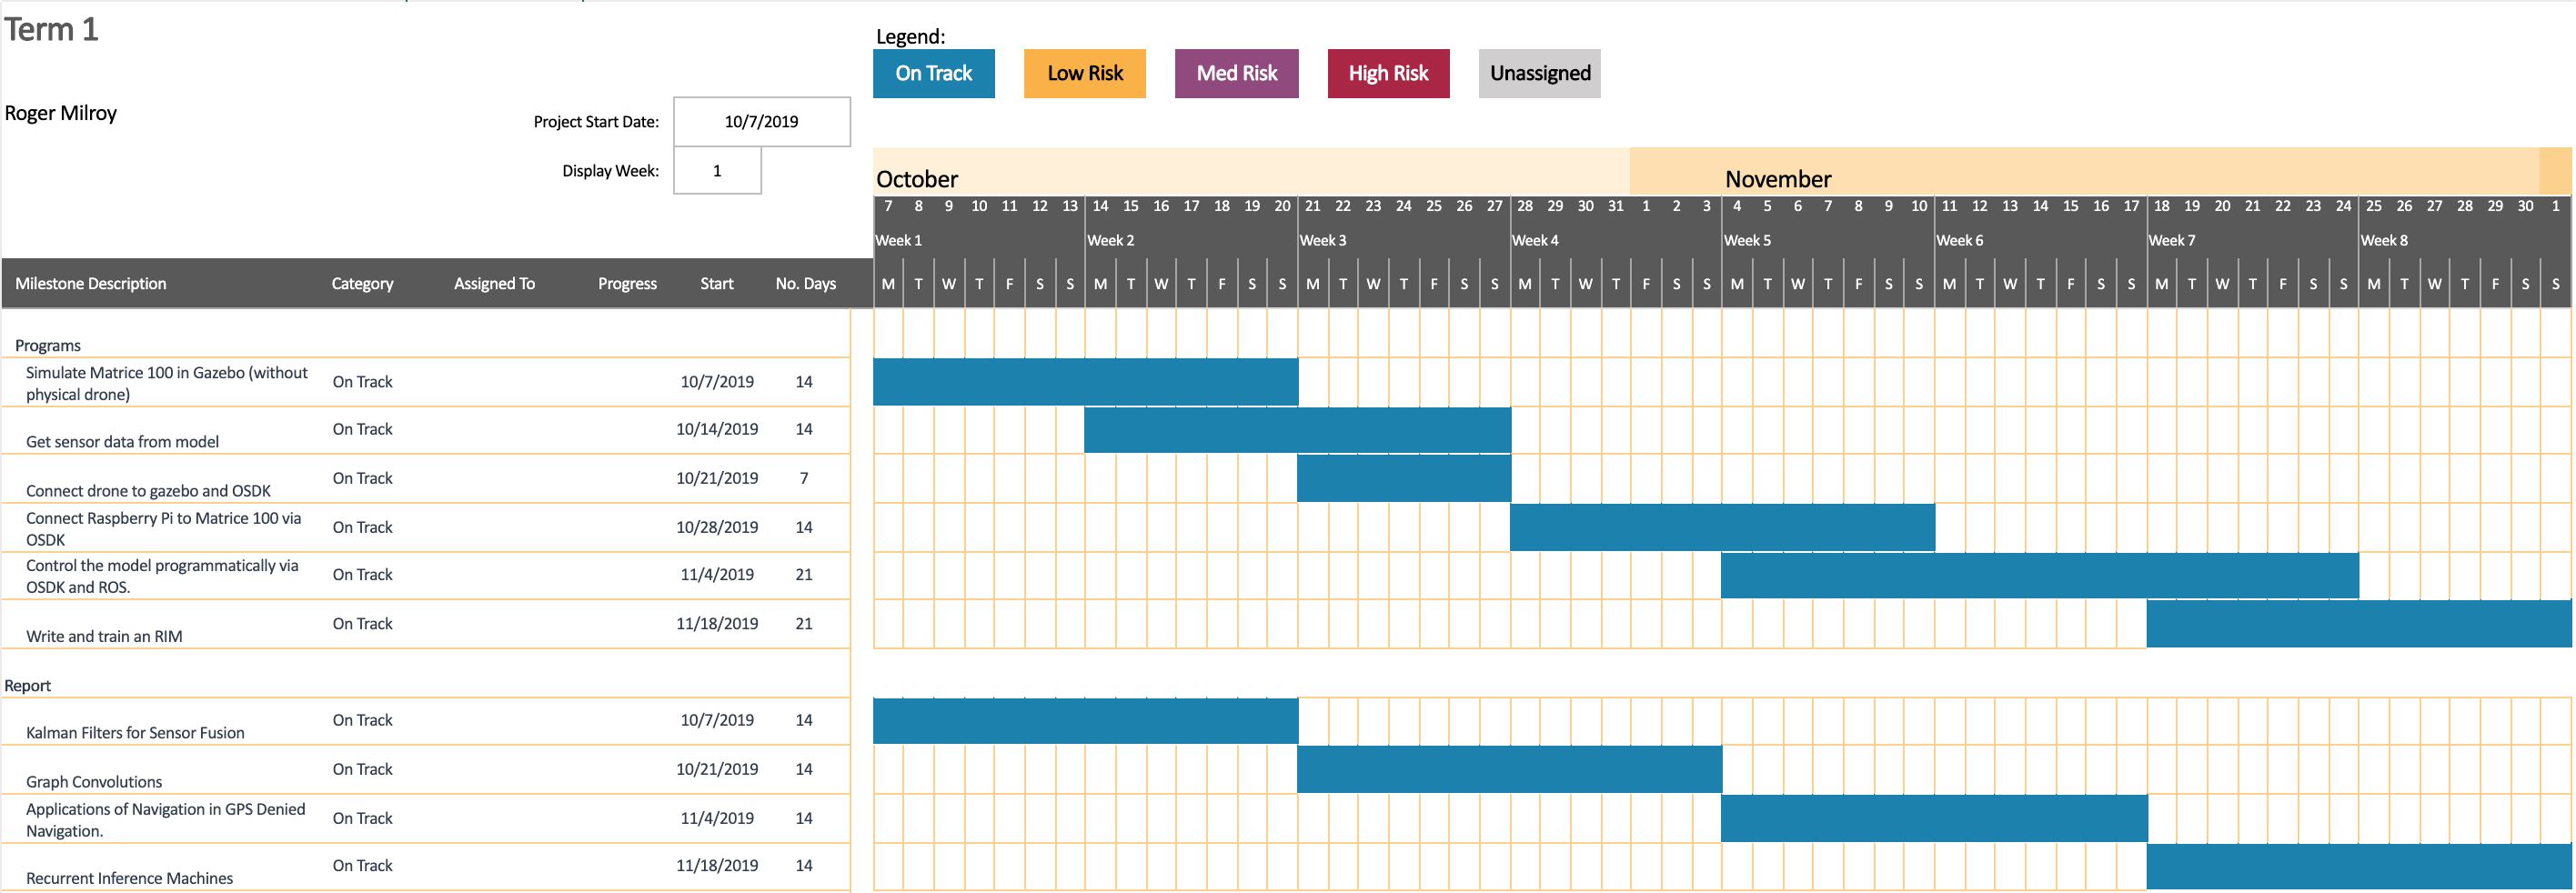
\includegraphics[width=\textwidth]{Term1Ganttv1.png}
  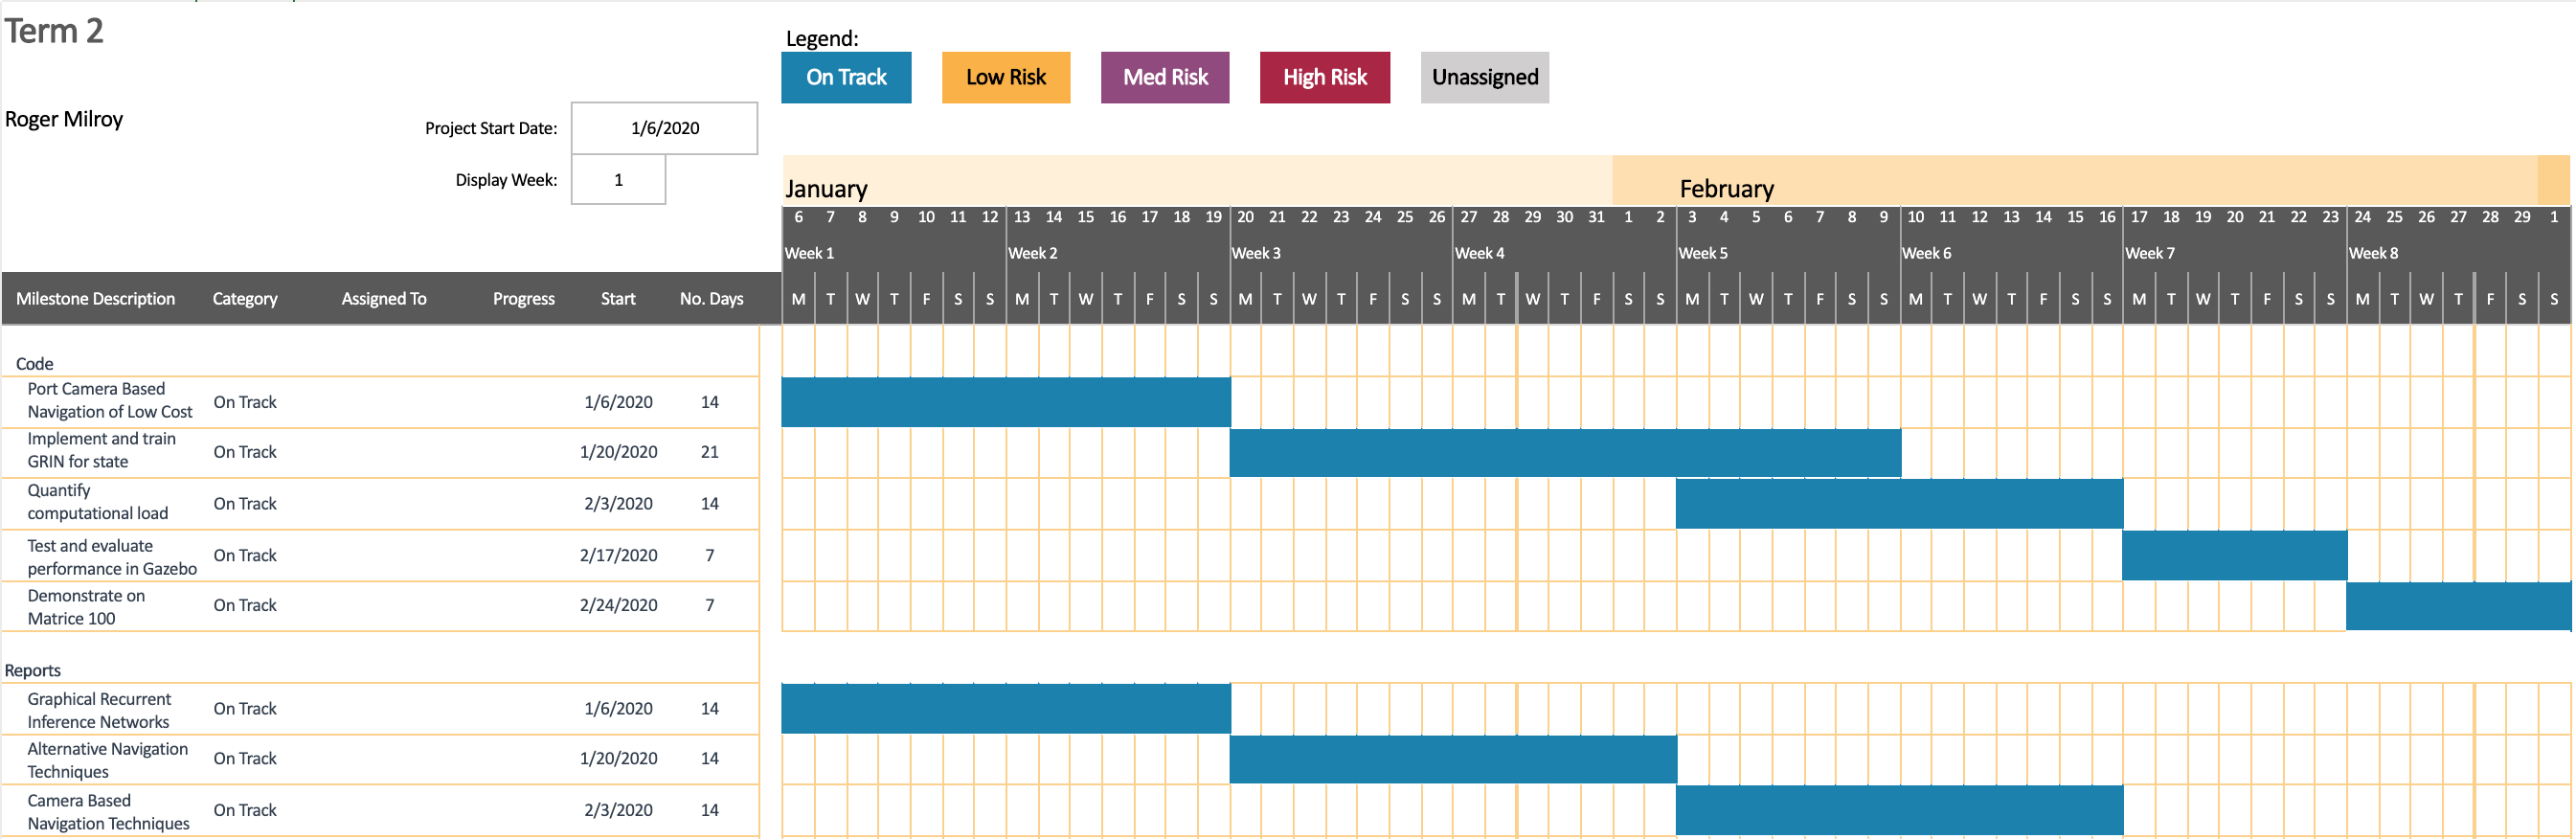
\includegraphics[width=\textwidth]{Term2Ganttv1.png}
  \caption{Original Plan Gantt Charts}
  \label{}
\end{figure}

\section{Revised Plan}

While working on the project the outlook changed quite significantly when I found the code for 
the Monocular SLAM with scale recovery was open source. This meant that I could directly build 
upon their work and extend it instead of spending the bulk of the project reimplementing their 
technique. This enabled me to pivot to focusing more on the implementation of HI. 
Under the new plan most of the first term is spent getting simulation working with the existing 
code base. I also implement a simple version of the HI technique on synthetic 
position data.


\begin{figure}[h]
  \centering
  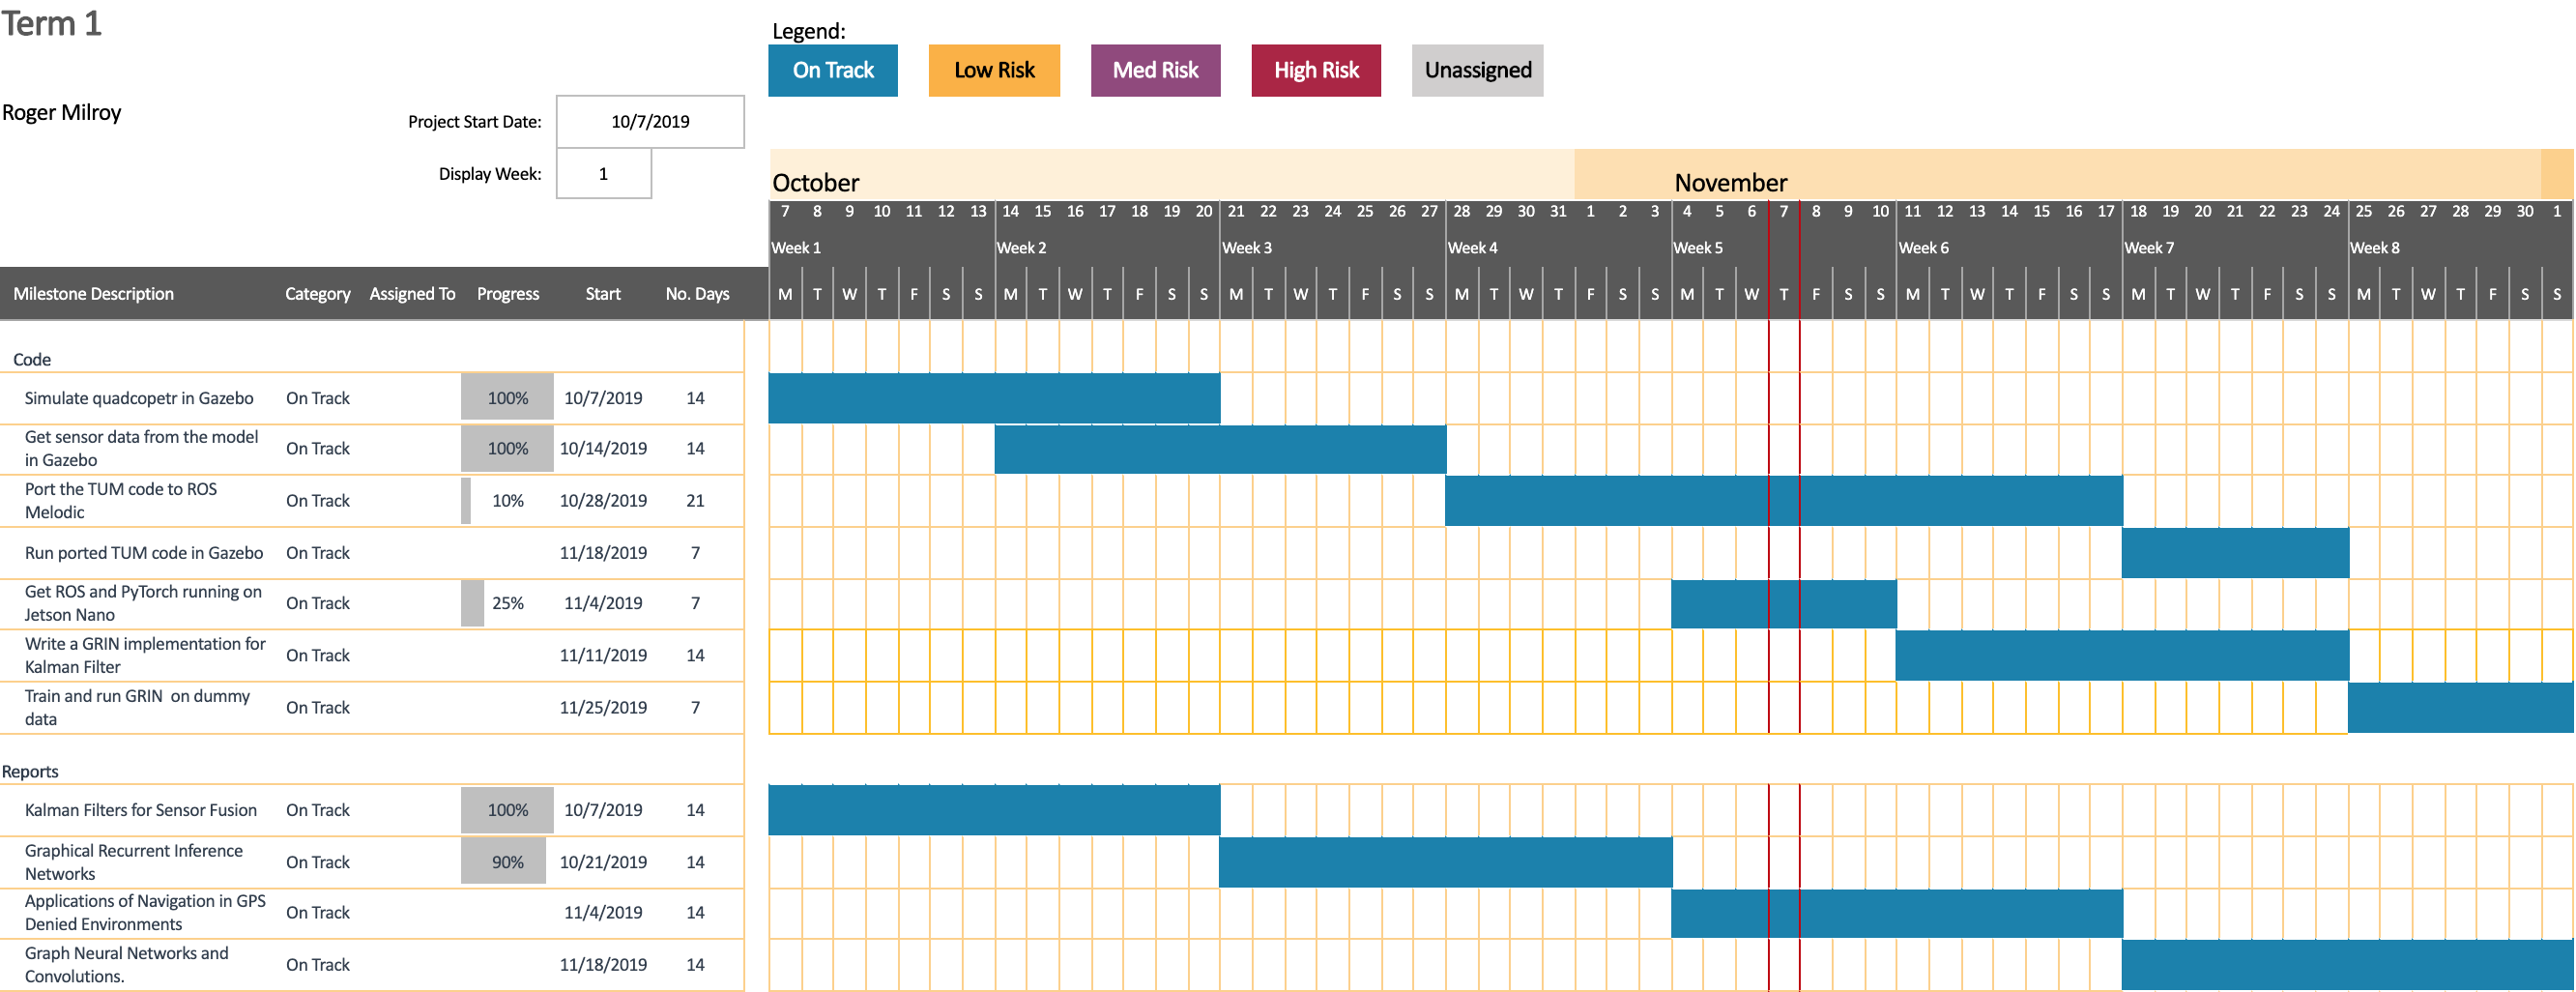
\includegraphics[width=\textwidth]{Term1GanttChart.png}
  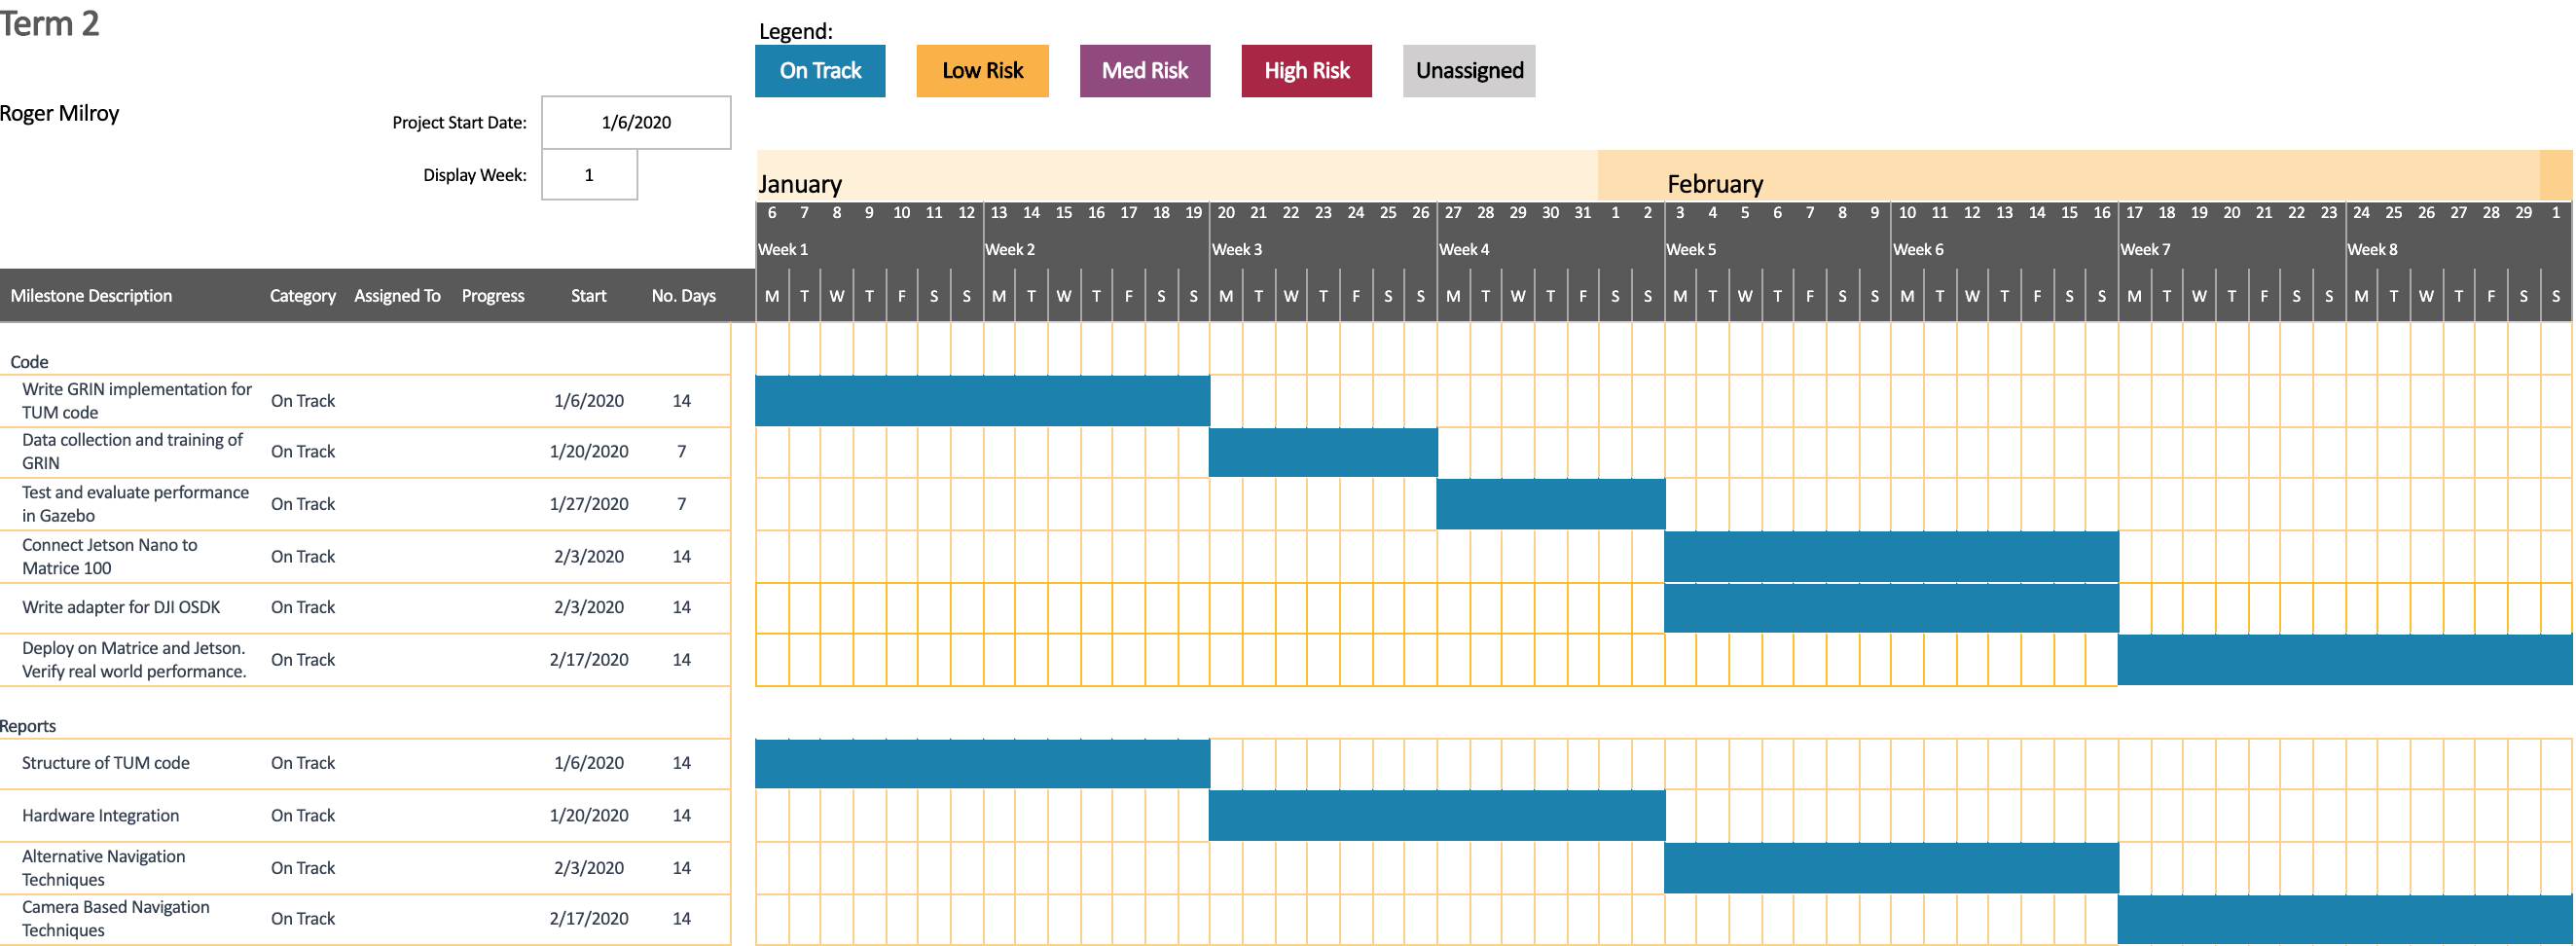
\includegraphics[width=\textwidth]{Term2GanttChart.png}
  \caption{Revised Plan Gantt Chart}
  \label{}
\end{figure}

%%%%%%%%%%%%%%%%%%%%%%
%%% Background Theory
\chapter{Background Theory}

\section{Gazebo and ROS}

%% Explainer on Gazebo and ROS and see if there are references for them.
In order to demostrate the effectiveness of the code that I have written it is essential that it is 
demonstrated first in a simulated environment. This neccesitates using Gazebo as it is the industry 
standard robot simulation software. In a similar token the industry standard robot development 
framework is ROS, which works with Gazebo and so this is the primary technology stack that I am 
using.

Both ROS and Gazebo are very powerful but they don't have a particularly easy onboarding process. 
For learning basic ROS concepts I used a service called Robot Ignite Academy that has some simple 
tutorials to make the process of learning the ROS way of doing things a bit quicker. One challenge I 
had at the very early stage was understanding what ROS actually was. There are very few high level 
descriptions of it, and they are certainly not the first topic on the ROS tutorials pages.

What I learned was that ROS is a paradigm of programming robots as well as an 
implementation of that paradigm. The paradigm is that each peice of code on the robot is a Node 
that takes data from a Topic, processes it and outputs data for other Nodes to use on a Topic. 
Some Nodes don't do both of these and some also directly effect change in the robot, think of a 
Node that controls a motor, it would read and change the voltage to the motor.

The other concepts that make up ROS are that of Services which are synchronous and Activities that 
are asynchronous, both operate on the Client - Server pattern. Topics as I mentioned are 
communication channels that operate on the Publisher-Subscriber pattern. And Messages which actually 
have quite a bit of intricacy and can be quite confusing. There are 3 types of Message. Regular 
Messages that are published to Topics. Then Actions and Services also define their own formats of 
messages. They will often use standard messages defined for use in Topics but additional message 
formats will be generated for each Action or Service.
%% Need to add references

\section{Monocular SLAM with scale recovery.}

%% put a UML diagram of the library layout/dependancies.
In two related papers \cite{Engel:FigureFlying}\cite{Engel:Camera-basedNav}, Engel et al. present a 
technique of Monocular SLAM that is able to recover absolute scale. In order to understand why 
this is significant and important some background is needed.

The primary problem of visual SLAM techniques is that of creating a high quality depth map of the 
surroundings. This can be accomplished by stereo vision, which is where two cameras are used and the 
distance and rotation between the two of them are known. Ideally the axes are aligned and there is 
no rotation between the cameras though this can vary depending on the specific requirements.
This can be extended to use three or more cameras but in the more general case, known as structure 
from motion, it is possible to use a single camera. In that case we are trying to recover the 
transformation and rotation between frames. This is possible however it is not possible to recover 
absolute scale from this technique as we don't know the absolute distances between frames. In the 
stereo case the information about the position and orientation of the cameras relative to each other
is known a priori and so we can recover absolute scale.

Engel et al. tackle the issue of scale recovery by using data from the IMU which usually consists of 
3 accelerometers and 3 gyroscopes and often a magnetometer or other absolute scale sensors such as 
altimeter or barometer. This is standard equipment on quadcopters as it is needed to maintain stability. 
They use the information provided by this sensor in conjunction with the structure from motion 
equations in order to recover the absolute scale. In order to estimate the scale factor which is 
usually referred to as $\lambda$ they take a maximum likelihood approach, which in simple terms 
means they estimate the $\lambda$ that maximises the likelihood of the $x$ and $y$ positions 
measured by onboard sensors. In order to solve successfully they turn it into the negative log 
likelihood which you then minimize. This is a common trick and in this case it leads to a closed 
form solution for $\lambda$. This is important as it reduces the computational cost and makes it 
more feasible with onboard computation. In the paper they use a Parrot AR drone which has very 
constrained payload and computation capacity so they use offboard computation.

In the second paper \cite{Engel:FigureFlying} they present the full system including the scale 
estimation and demonstrate its effectiveness in position flying and holding.


\section{State Estimation}

%% Kalman Filters
The core method used for state estimation in the face of noisy sensors is the Kalman Filter. It is 
used by Engel et al.\cite{Engel:Camera-basedNav} for state estimation and sensor fusion which are 
its most common uses in this field.

Let us formally define the problem. The system we are measuring is assumed to be characterised by a 
Hidden Markov Model, this is how Kalman characterised the dynamical system we are interested in \cite{Kalman1960ANA}. 
In this formulation there are hidden states $x$ and observations $y$. The system being a Hidden 
Markov Process means that it is characterised by the following equations:

\begin{align}
  x_t &= Ax_{t-1} + Q_t \\
  y_t &= Hx_t + R_t
\end{align}

Where $A$ is the transition matrix from time $t-1$ to $t$, and $\xi_t$ is the noise at time $t$. 
This represents that the model dynamics are stationary so $A$ is fixed but there is noise in 
transitions, that is transitioning between states is non-deterministic. $H$ is the measurement 
matrix and $R_t$ is the noise in the measurements. This models the reality of noisy measurements 
that may not be correct and in fact represents the true problem. We want to recover the true 
measurements despite being given noisy observations.

The Kalman Filter gives an optimum estimate of $x$ which I will call $x^*$ by deriving three matrices 
$\Phi^*$, $P^*$ and $\Delta^*$:

\begin{align}
  \Delta^*(t) &= A_{t+1;t}P^*_tH^T_t[H_tP^*_tH^T_t]^{-1} \\
  \Phi^*_{t+1;t} &= A_{t+1;t} - \Delta^*_{t+1;t}H{t} \\
  P^*_{t+1} &= \Phi^*_{t+1;t}P^*_tA^T_{t+1;t} + Q{t}
\end{align}


Note that in the Kalman formulation he also considers non stationary dynamic systems. In our 
situation we assume stationarity which allows us to drop the time specification on the transition 
matrices $A$ and $H$.

With these matrices, the optimal estimate of state at time $t+1$, $\hat{x}_{t+1|t}$ is given by 

\begin{align}
  \hat{x}_{t+1|t} &= A^*\hat{x}_{t|t-1} + \Delta^*_ty_t
\end{align}

The estimation error $x'$ and covariance of the error, cov $x'$ are

\begin{align}
  x'_{t+1|t} &= A^*x'_{t|t-1} + Q_t \\
  \text{cov } x' &= P^*_t
\end{align}

From this we can see that the Kalman Filter is an iterative process where each iteration builds upon 
the previous best estimate of state. To recover the estimates of the true measurements we simply 
need to multiply the best estimates of the state by the measurement matris $H$.

Kalman and Bucy extended the Kalman filter that, in the form stated above works for discrete time, to the 
continuous case the year after the original paper \cite{Klmn1961NewRI}.

These equations only apply to linear dynamic models which is something of an issue given that most 
real life applications are of non linear dynamic systems. To solve this we use Taylor expansions to 
linearise our non-linear models around the current state \cite{ExtendedKalmanNasa}. This does 
unfortunately add a large overhead as we need to re linearise at each time step to avoid 
accumulating linearisation errors.

%% Graph Neural Networks
\section{Graph Neural Networks}

% Explain the premise behing GNNs
As the technique I am implementing makes use of Graph Neural Networks (GNNs) I will first explore
what GNNs in relation to regular neural networks (NNs).

\subsection{Neural Networks}
To understand GNNs it is first necessary to understand some basic things about NN and some of 
their properties. Firstly the paradigm of learning that NNs fall under to is called representation learning. That is learning
meaningful representations of data in order to achieve some useful outcome.

Secondly is that NNs are Universal Function Approximators \cite{Hornik}.
That is given sufficient hidden layer neurons a neural network can approximate any real valued function 
no matter how complex. This is the basis for their power and flexibility.

This doesn't come without drawbacks however. The cost of this flexibility is that 
training a universal function approximator (or a feed forward network with an arbitrarily 
large hidden layer) is not necessarily feasible in computational terms or in terms of 
the amount of data required. 

In order to overcome this limitation there has been great progress in 
formulating specific architectures of neural networks. Some good examples of these 
are Convolutional Neural Networks (CNNs) and Residual Networks (ResNets). 
One of the keys to these models successes is that they constrain the neural architecture.
For these two in particular they constrain the model to Euclidean space and 
particular dimensions within this space. This restriction means that 
the resulting network is no longer a universal function approximator but that 
also reduces the amount that the network has to learn like about the rules of Euclidean space and what
a dimension within the data is. It is precisely these restrictions that 
enable such networks to learn with fewer data samples and to a greater accuracy
than would be possible otherwise.

This can be rephrased with a slightly different interpretation by seeing the constraints on
the network as introducing inductive biases into the model. This biases it to learn
certain features of the dataset and not others. 

\subsection{Graphs}

% Define Graphs?
We define graphs as a collection of nodes (also known as vertices though I will use the word node from now on) 
and a collection of edges over those nodes.
Graphs are prevalent across many different areas of science and are a particular focus of
many Computer Scientists. Famous examples of graph algorithms include Djistra's Algorithm, Depth First Search and A star.
Why are graphs so prevalent? Well the answer is that they have great expressive power to 
represent objects or concepts and their relations.

The flexibility of graphs is mirrored in the great variety of operations that we might want 
to carry out over them. At the same time there is a huge number of different configurations 
of graphs varying over degree of connectivity of each node, whether edges are weighted or directed, 
containing cycles or not and whether the graph changes at all.
Whether the edges represent different kinds of relation and what information each node contains.

\subsection{Graph Neural Networks}

We consider each node to have a vector label or feature. This may contain information about edges or not.
If we were to try and apply CNNs or RNNs to graphs in this form, we could do so by stacking the node 
features and operating over that. In this case the node features would contain the information about edges.

This is not ideal because it enforces or biases the model to a particular ordering of nodes where there 
might not be one. We could overcome this by computing over all possible orderings of nodes.
This would however add significant computation. \cite{graphoverview}
It also prevents the model from exploiting the graphs inherent structure, as it had been 
folded into the nodes themselves. It is clear then that this is not the best approach.

% GNN
\subsubsection{Original GNN}
Now I will explain the original GNN proposed by \cite{GNN}. The following explanation is drawn from \cite{graphoverview} with some rewording. 
The goal of the GNN is to learn an embedding $ \emph{h}_x \in \Reals_s $ of each node $x$ which contains the information 
from the node and its locality. This embedding is then used to generate an output $\emph{o}_x$ of each node, often called the decoding step,
where the embedding of each node generates a prediction of some kind for example the node labels.

In order to compute these embeddings and outputs we define two parametric functions, the first is $f$ a 
local transition function which is shared by all nodes, and $g$ the local output function. These are defined as:

\begin{align}
  \textbf{h}_v &= \emph{f }(\textbf{x}_v, \textbf{x}_{co[v]}, \textbf{h}_{ne[v]}, \textbf{x}_{ne[v]})\\
  \textbf{o}_v &= \emph{g }(\textbf{h}_v, \textbf{x}_v)
\end{align}

where $\textbf{x}_v$, $\textbf{x}_{co[v]}$, $\textbf{h}_{ne[v]}$, $\textbf{x}_{ne[v]}$ are the features of v, the features of its edges, 
the states, and the features of the nodes in the neighborhood of $v$, respectively.

This can be condensed by stacking vectors to form matrices. Then we have $\textbf{X}$, $\textbf{X}_N$, $\textbf{O}$ and $\textbf{H}$ 
consisting of all features, the features of the nodes, the outputs and the states respectively. In this form we then have global transition 
function $F$ and global output function $G$.

\begin{align}
  \textbf{H} &= F(\textbf{H}, \textbf{X})\\
  \textbf{O} &= G(\textbf{H}, \textbf{X}_N)\\
\end{align}

The GNN takes inspiration from Banach's fixed point theorem \cite{khamsi_kirk_2011} and uses the following iterative scheme to 
compute the states:

\begin{align}
  \textbf{H}^{t+1} = F(\textbf{H}^t, \textbf{X})
\end{align}

This converges to a stable $H$ exponentially fast for any start point of $\textbf{H}_0$

We use NNs for the parameterised functions $\emph{f}$ and $\emph{g}$.

As stated in \cite{GGNN} the model is trained using the Almeida-Pineda algorithm \cite{Almeida}\cite{Pineda} where 
the states are computed to convergence at which point the output and losses are computed. 
The gradients of the weights in the transition function and output fuction networks are computed from
this final state and the weights updated according to the optimisation algorithm selected.


% Adding Recurrence.
\subsubsection{Recurrence}

An extension or variation of the GNN is the Gated Graph Neural Network (GGNN). The key reason for the introduction
of the GGNN is to reduce the restrictions on the transition function. Rewording what was stated in \cite{GGNN} the 
paper that proposes the GGNN they outline the challenge of the original GNNs learning scheme.
As I just described, in the regular GNN the loss and gradients are computed relative to the final converged state.
This requires that the parameters of the NNs be constrained so that it is a contraction map, otherwise convergence cannot be
guaranteed. In order to remove this restriction, as there is evidence that long range dependencies ar lost in the
contraction map scheme, they add a Gated Recurrent Unit (GRU) \cite{GRU}. In this situation
information is conserved at each time step and while gradients are still computed from the
final state and output, the GRU is unrolled backpropagated through time (BPTT) \cite{Pineda} is used to propagate these
gradients across all time steps of the iterative procedure. This removes the constraint on the parameters of the
component NNs.


% MPNN
\subsubsection{MPNN}

After the introduction of the GNN there have been many additional variants have been proposed
such as Spectral Networks and Graph Convolutional Networks (GCN) and Graph Attention Networks.

There have been proposed some frameworks that generalise these various variants of GNNs.
The framework relevant to this application is called the Message Passing Neural Network (MPNN) which was proposed by \cite{mpnn}.

Again I am using the explanation of \cite{graphoverview} with some rewording as it is an excellent high level explanation.

The MPNN has two phases, the message passing phase and the readout phase. The message passing phase runs for $T$ steps and there are two parts 
the message function $M_t$ and the update function $U_t$, $\textbf{e}_{vw}$ is the edge feature on the edge from $v$ to $w$.

\begin{align}
  \textbf{m}^{t+1}_v &= \sum_{w \in N_v} \emph{M}_t(\textbf{h}^t_v, \textbf{h}^t_e, \textbf{e}^t_{vw})\\
  \textbf{h}^{t+1}_v &= U_t(\textbf{h}^t_v, \textbf{m}^t_v)
\end{align}

The readout phase computes a vector for the whole graph using the readout function $R$ and $T$ denotes the total number of time steps or iterations.

\begin{align}
  \hat{\textbf{y}} &= R({\textbf{h}^T_v | v \in G})
\end{align}

This is modifiable of course to allow a per node output. In this case the readout function would be 
similar to the output function of the original GNN. In fact there are many parallels between the 
original GNN and the MPNN but the MPNN has more flexibility which allows it to capture 
the majority if not all of the supervised variants of the GNN.

We can also implement the GGNN using this framework.


%% Hybrid Inference
\section{Hybrid Inference}

Now I introduce the technique that form the core objective of this project, Hybrid Inference. First 
introduced in \cite{Satorras2019CombiningGA} which also gave examples on Lorenz attractors and 
Kalman filters. While Kalman Filters give optimal estimates in the face of noise, it is almost 
impossible for them to be completely precise due to that noise. This we can see by observing the 
error in the estimates at each time step.

Absent an accurate fix of state, ie. a noiseless measurement, the error grows 
continuously to the point where estimates may no longer be meaningful.

At the same time it is now possible to train a neural network to directly estimate position given
noisy inputs \cite{NNStateEstimation}. The concept of Hybrid Inference is to leverage the relative 
strengths of pre-existing knowledge, in this case the Kalman Filter that accurately describes the 
behaviour of linear or linearised dynamic models up to a degree of error, and Deep Learning techniques 
that are able to model highly non linear systems but require large amounts of data to train.
In the Hybrid Inference model, expert knowledge is incorporated by integrating the model of the 
system with a Graphical Neural Network (GNN) modelling the residual error to improve accuracy above what is possible with a 
Kalman filter alone.


Reexamining the problem solved by the Kalman filter, Satorras, Akata and Welling reformulate the 
problem to be a maximum likelihood problem\cite{Satorras2019CombiningGA}.
Where the states are $\mathbf{x} = \{x_0, x_1 ... x_k\}$ and the observations are $\mathbf{y} = \{y_0, y_1 ... y_k\}$
In this context, the task is to predict the optimal estimate of $\mathbf{x}$, $\mathbf{\hat{x}}$ which is defined as

\begin{align}
  \mathbf{\hat{x}} = \underset{x}{\text{argmax}}\ p(\mathbf{x}|\mathbf{y})
\end{align}

Again as we assume a Markov process and that the transition is stationary this can be expressed as 

\begin{align}
  p(\mathbf{x},\mathbf{y}) = p(x_0)\prod_{t=1}^T p(x_t|x_t-1) p(y_t|x_t)
\end{align}

They model this as an iterative optimization process to arrive at $\mathbf{\hat{x}}$
Specifically they define a recursive update operation for the general case and then formulate it 
for the Hidden Markov case

\begin{align}
  x_t^{(i+1)} = x_t^{(i)} + \gamma M_t
\end{align}

Where $M_t$ represents the sum of matrix products, which they call messages, from $x_t-1$ to $x_t$ 
from $x_t+1$ to $x_t$ and from $y_t$ to $x_t$.

In our case these messages turn out to be

\begin{align}
  x_{t-1} \rightarrow x_{t} &= -Q^{-1}(x_t - Fx_{t-1}) \\
  x_{t+1} \rightarrow x_{t} &= F^TQ^{-1}(x_{t+1} - Fx_t) \\
  y_t \rightarrow x_t &= H^TR^{-1}(y_t - Hx_t) 
\end{align}

% \begin{wrapfigure}{r}{0.25\textwidth} %this figure will be at the right
%   \centering
  
% \end{wrapfigure}

The graphical interpretation is of the $x$s and $y$s at each time step forming nodes in a graph. The 
edges are the same as the direction of the messages, that is from $x_{t-1} \rightarrow x_t$, $x_{t+1} \rightarrow x_t$ and $y_t \rightarrow x_t$. 
The messages passed over these edges iteratively update the $x$s and after some iterations they 
converge to a best estimate.

%% Insert a graph here.

\begin{figure}[h]
  \centering
  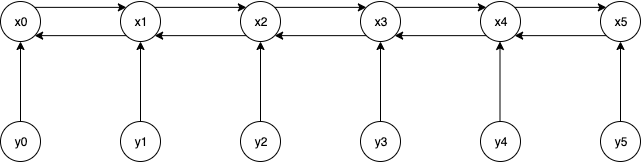
\includegraphics[width=0.8\textwidth]{GraphicalKalmanModel.png}  
  \caption{}
  \label{}
\end{figure}

This graphical interpretation allows us to define an equivalent graph with different dimension nodes 
but the same edges. These are known as $h_x$ and $h_y$ which stands for hidden nodes relating to $x$ 
and $y$ respectively. 

%% Insert another graph here.

The key part of the paper is to define a GNN that operates over this graph with a message passing
routine over the nodes that connect edges and the messages passed in the original 
graph. More specifically for each type of edge, for example $y_t \rightarrow x_t$, we define a 
feedforward neural network that takes the source node, the target node and the message and outputs 
an encoding of the edge, I will refer to these as edge models. These encodings are summed according 
to their source node and then passed through a separate feedforward network which I will call the 
node model. 

The output of this is passed through a GRU along with the previous $h_x$ in order to produce a new 
estimate of $h_x$. The interpretation of this is that edge feedforward networks compute the residual 
error over the edges, the node model computes the residual error left in the $h_x$ and the GRU allows 
some of the past residual error to propagate into the current estimate. The final step passes the new 
$h_x$ through a decoding step to produce an additional corrective factor in addition to $M_t$ called $\epsilon$.

This gives us the final general recursive update rule

\begin{align}
  x_t^{(i+1)} = x_t^{(i)} + \gamma (M_t + \epsilon_t)
\end{align}


\section{My Contributions}

% Some discussion of what I have accomplished. 
% from the booklet "an interesting discussion on what you have achieved in a more global context"

In the HI paper they implement a Kalman Smoother over linear and non linear systems however in both of these cases
they didn't cover the case of having inputs to the system. 
%  or using the technique for prediction.

This is necessary in order to be useable in the context of drones as there are inputs required at 
every point, both to maintain stability as well to navigate or accomplish anything useful.

In order to use HI on MAVs in reality it is also necessary to be able to predict a short way 
into the future, that is to implement a true Kalman Filter rather than just a Smoother, the distinction
is quite important, a Smoother operates only on timesteps prior to the current measurement and a Filter 
operates on the current measurement as well as future time steps without measurements (by omitting the update step). 
In order to control a drone effectively you need to account for the fact that there will be time lags in some 
parts of the system. For this reason you need to be able to predict a short way into the future for the most effective control.


% Change to the probability function
\subsubsection{Inputs}

To add inputs I needed to change the probability distribution we are modelling.

\begin{align}
  \hat{\textbf{x}} = \underset{\textbf{x}}{\text{arg max }} p(\textbf{x} | \textbf{y}, \textbf{u}) 
\end{align}
where $\textbf{u}$ are the inputs.

This changes the recursive update function (Eq. 5 in \cite{Satorras2019CombiningGA}) to be 

\begin{align}
  \textbf{x}^{(i+1)} = \textbf{x}^{(i)} + \gamma \nabla_{\textbf{x}^{(i)}}log(p(\textbf{x}^{(i)} | \textbf{y}, \textbf{u}))
\end{align}

% Change to the messages

Which in turn changes the derived input messages to be 

\begin{align}
  \mu_{x_{k-1} \rightarrow x_k}^{(i)} &= \frac{\partial}{\partial x_k^{(i)}} log(p(x_k^{(i)}|x_{k-1}^{(i)}, u_{k})\\
  \mu_{x_{k+1} \rightarrow x_k}^{(i)} &= \frac{\partial}{\partial x_k^{(i)}} log(p(x_{k+1}^{(i)}|x_{k}^{(i)}, u_{k})\\
  \mu_{x_{y_k} \rightarrow x_k}^{(i)} &= \frac{\partial}{\partial x_k^{(i)}} log(p(y_{k}|x_{k}^{(i)})
\end{align}

% Change to the derived matrix operations.

Formulated for the Kalman filter model this gives us

\begin{align}
  \mu_{x_{k-1} \rightarrow x_k}^{(i)} &= -\textbf{Q}^{-1}(x_k - (\textbf{F}x_{k-1} +\textbf{G}u_k))\\
  \mu_{x_{k+1} \rightarrow x_k}^{(i)} &= \textbf{F}^T\textbf{Q}^{-1}(x_{k+1} - (\textbf{x}_k + \textbf{G}u_{k+1}))\\
  \mu_{x_{y_k} \rightarrow x_k}^{(i)} &= \textbf{H}^T\textbf{R}^{-1}(y_k - \textbf{H}x_k)
\end{align}

Where $\textbf{G}$ is the gain matrix over the inputs $u$.

In a wider context this is a small but significant extension that shows that this technique
could be used in the full spectrum of applications of the Kalman Smoother. 

I detail the implementation in Work Completed and share the results which are comparable 
with the original HI implementation.

% Extension to prediction.

\subsubsection{Prediction}

Extending to prediction is a different challenge. I elected to take the simplest approach
which coincidentally is analagous to the approach that the KF takes for prediction.

I augment the sequence over which the technique operates for smoothing with O values for 
measurements or $y$s. This is analagous to running the predict steps of the KF with no update step.
The sequence is again iteratively optimized to arrive at the estimates of the future states.

%% ADD MATHEMATICAL REPRESENTATION HERE.


%%% Software Engineering
\chapter{Software Engineering}

\section{Tools}

\subsubsection{Version Control System}

I used git as my version control system, and GitHub as my remote. I actually have a number of 
repositories because for the ROS section of the project it was necessary to modify existing 
projects code. I created a private fork of the relevant projects and then modified them as necessary.

I have separate branches for development, reports and for each feature that I am working on. 
These last ones are only temporary and are closed as soon as the feature is tested and integrated 
back into development. The workflow that I have decided upon is to use development for completed 
features once they have been tested. This does not imply that development is stable however so I 
only release code considered stable to master. The idea is that master should only contain stable 
code and be safe to use at any point.

\subsubsection{Project Task Tracking}

I used Trello in order to organise and keep track of tasks while completing them. I used a single 
board with To Do, Doing and Done lists. Each task is a card and has an associated due date.
This is really useful to stay on track and quickly assess the state of the project at a glance. 
I also used this while replanning as I could evaluate each task and see whether it was still 
relevant in the new context. One additional advantage of using Trello is that it keeps track of 
history and has space for lists within tasks allowing them to be broken up into sub tasks.

%%%%%%%%%% Add a screenshot? %%%%%%%%%%%%%%%


\subsubsection{Development Support Tools}

IDEs support efficient coding with a number of useful tools and features. The primary advantage 
is the code completion support. This greatly speeds development, especially in more verbose 
languages. One of the most valuable features in the context of this project is the debugger.
This allows the developer to step through the program where necessary and inspect each variable
as it changes. This was particularly useful in the implementation of HI as the dimensions of the
tensors at each step is extremely important and often hard to keep track of. Interestingly 
this particular issue has caused PyTorch to add support for named tensors. This allows each 
dimension to be named, which mostly solves the problem.

I used VSCode, CLion and PyCharm as Development Environments. They each have different advantages 
and disadvantages and I used VSCode and CLion for the C++ work and PyCharm for the Python work.

For ROS development I have an Ubuntu VM with the relevant dependencies installed as well as the 
IDEs I just mentioned. ROS uses catkin for building projects which in turn builds upon CMake.
I used UMLet for drawing up the UML diagrams 

For testing I used the built in testing framework for Python, 'unittest'. This provides a very 
similar framework to JUnit and allows for clear easy test setup and management.


\section{Design and Testing Strategy}

\subsection{Design}
% ROS

This project has been different to most projects that I have worked on to date in terms of software 
design. Most projects have been implementing from scratch using some different technologies but 
either very little or none in terms of pre existing code base. This gives a lot of freedom and 
control to the design.

In this project it has been quite different. I have been working with pre existing code bases from 
TU Munich and TU Darmstadt. This has constrained the design and implementation of these parts 
of the project. Outside of these sections the goal of all the design decisions has been modularity 
and reusability. In some cases this has not been possible due to constraints of the technologies
that I have been working with.

In terms of overall development approach I have followed Test Driven Development (TDD) where possible.
This has been naturally limited in the ROS sections to within node testing. Each component of the nodes 
has been unit tested where possible with integration testing being carried out in an incremental
fasion during the development process.

It is widely accepted that good code should be modular and reusable where possible. There are 
aspects where this is obviously not possible, such as configurations and any implementation 
specific work, but this should where possible be isolated and offer abstract interfaces.

With respect to the packages I have chosen, the hector stack and the TUM work, they have to some 
extent taken this approach but only really within the project. 
This complicates my work somewhat but at the same time using these as the base allows me to explore
more advanced concepts over reimplementing the functionality of these modules. It has forced me to 
adapt my natural coding style to fit in with the pre existing code and conventions established within
them. 

For the HI implementation section of the project, I separated the Graphical and GNN parts of the implementation.
They became separate classes that had defined intefaces for the forward methods that were as stable as possible.
They are composed into the final HI implementation, this has risks of high coupling which I mitigated as 
far as possible by keeping the intefaces (primarily the forward method) as stable as possible in terms 
of inputs and return values. This allows the internal structure to change without the HI implementation 
being modified at all.

I added interfaces for predictor and smoother in order to further enforce this principle. There are 
some limitations to this due to the fact that HI works with multidimensional tensors and dimensionality 
makes a large difference. I would ideally be able to prescribe the dimensionality of the inputs and 
return values from each function. Unfortunately there is no mechanism for that in any language or 
framework at this time.

When it came time to integrate HI into the hector stack I needed to port the PyTorch implementation of 
HI to run in C++. This required various changes to make the implementation serialisable with the 
TorchScript compiler module. Some of these overrode design decisions I had made earlier.

While integrating HI into the hector stack, I was much more restricted in the design choices I could 
make as I had to work inside the structure that was already established. Specifically I had originally 
planned to implement the HI as a ROS node to minimise coupling. The hector stack decided not to take 
that approach for pose estimation, I believe due to latency concerns. So I directly subclassed their
Filter base class modelled on their EKF implementation. I did this so that they could be easily 
swapped to provide comparison.

\subsection{UML}
%% UML

%%%%%%%%%%%%%%%%%%%%%% OLD %%%%%%%%%%%%%%%%%%%%%%%%
I have included the package diagram that describes the high level design 
of the project as well as the class diagram of the HI demonstrator.

\begin{figure}[h!]
  \centering
  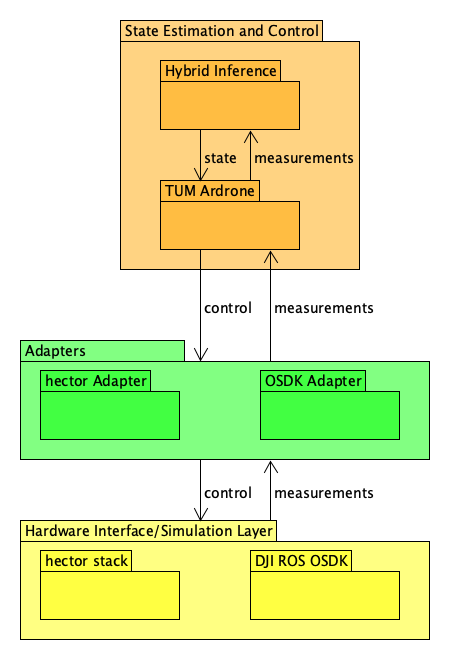
\includegraphics[height=0.30\textheight]{hybrid-inference-package-uml.png}  
  \caption{Package diagram of the project.}
  \label{}
\end{figure}

\begin{figure}[h!]
  \centering
  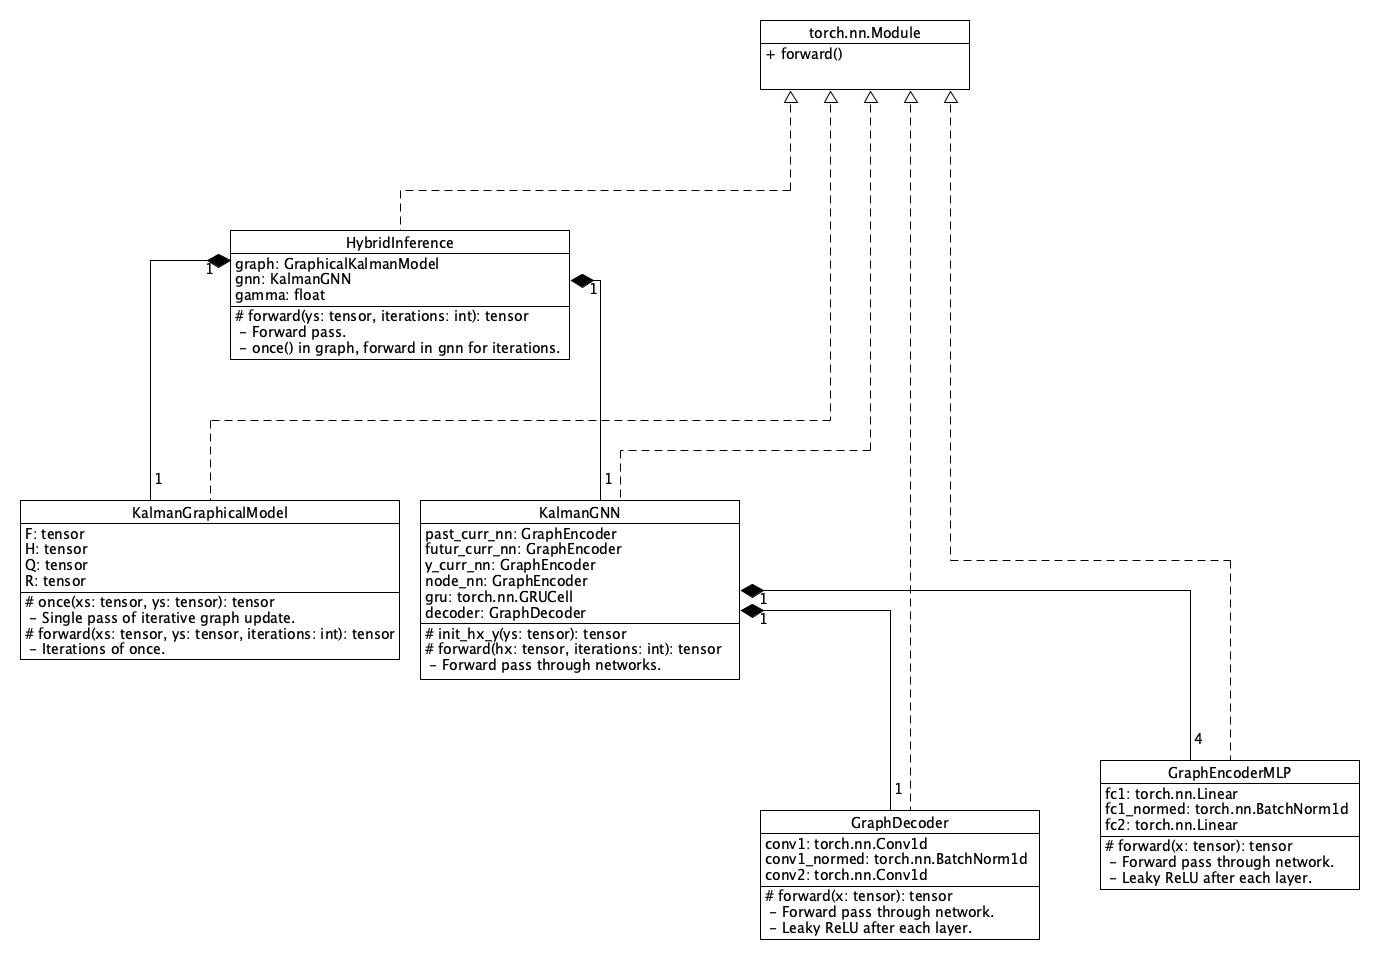
\includegraphics[height=0.36\textheight]{hybrid-inference-uml.png}
  \caption{Class diagram for Hybrid Inference}
  \label{}
\end{figure}

\subsection{Testing Strategy}


%%%%%%%%%%%%%%%%%%%%%%%%%%%%%%%%%%%%%% MOOOOOOOORE %%%%%%%%%%%%%%%%%%%%%%%%%%%%%%%%%

The primary strategy that I have used for testing in this project is that of Unit Testing as much
of the components as possible while incrementally and continuously testing the integration of the
various components while developing. There has been a tight cycle of development and testing.

There have been some limitations to my ability to Unit Test everything, mostly due to using external
code bases. Having said that, I have thoroughly Unit Tested the proof of concept of HI, the Dataset
and Linear Motion model, as well as the extension to accept Inputs and Prediction.

\section{Development}

This section details the process of development that I went through. It is broadly organised by 
component and within component in chronological order.

\subsection{Hardware}

%% evaluation of alternatives
My original plan was to use a Raspberry Pi for onboard computation for transitioning to 
operating on the physical drone rather than in Gazebo. This was for a couple of reasons, primary was 
the low power draw while still offering gigahertz computation. I have a Raspberry Pi 2 and I planned 
to purchase a Raspberry Pi 4 for the final implementation due to its increased compute power.

%% selection of Jetson Nano
While experimenting with my RasPi 2 I found some limitations with its implementation of Python as 
well as concerns about its prospective performance due to reports found online. I researched 
alternatives, as there are a wide variety of Single Board Computers on the market now. While looking 
I found that NVIDIA produce the Jetson Nano and specifically the SDK kit, which is very similar to 
the RasPi but has native support for PyTorch, the deep learning library I am using as well as having 
128 GPU cores. This enables me to take advantage of parallelised matrix computation with the 
associated performance improvements. On top of this it only consumes up to 10W of power, admittedly 
this is double the 5W draw of the RasPi but 10W is the maximum, not necessarily what it will consume. 
I will explore power consumption in the second part of the project.

%% installation of PyTorch and ROS.
After the Nano arrived I installed PyTorch and ROS onto it. This allowed me to verify the steps 
needed for installing both packages and ensure the most streamlined set of instructions.

There were some issues with the original version of PyTorch installed due to the Nano using
an ARM CPU. This means that it has the aarch64 architecture and so compiled executables are trickier
to get hold of and often are not quite the same as x86. In this case PyTorch uses some external 
libraries for some of the matrix operations, these include OpenBLAS and MKL. In the first version 
I installed these were not present, preventing matrix inverse operations. This is critical 
to both Graphical Kalman Smoother and by extension the HI implementation.

I tried a number of solutions including installing from source however in the mean time an updated
version of PyTorch was released for the Nano which included OpenBLAS solving the problem.

In the end there were a number of factors that prevented the eventual hardware integration.

% I will still try and profile the time and power requirements of running the code for SLAM.

\subsection{ROS and Gazebo}

%% install ROS and Gazebo
The first task to carry out was to install ROS and Gazebo. As mentioned earlier ROS is the framework 
into which my code will fit. Gazebo is a simulation tool that I will be using to verify everything 
before deploying anything in reality. Luckily Gazebo is included with ROS (with some exceptions) so 
installing it separately is not necessary. If you need the most recent version of Gazebo this is not 
true, you need to follow some additional steps to install it and link it with ROS so they interact 
correctly.

I did have some confusion about which version of ROS I needed to be compatible with various things 
but I made the decision to stick with the most recent version of ROS and the standard version of 
Gazebo packaged with that. This simplifies the setup for anyone seeking to reproduce this project.

The ROS website\cite{melodic/installation/ubuntu} has an excellent guide on installing ROS for the 
first time on Ubuntu and I highly recommend it.

%% install hector code

After that I installed the hector stack. This was quite a long process of trial and error as there 
does not seem to be a guide for getting started with this set of packages. I first tried to install 
them from apt as they are available there. That did not work and I believe the issue is that they 
were built for an earlier version of ROS but packaged for melodic without any changes. Regardless 
of the reason that did not work. I was trying to install the hector quadrotor and hector gazebo 
packages as those were the only packages that I believed that I needed. I tried to clone them into 
the src folder of my catkin workspace. While trying to build it failed because of dependencies on 
other hector packages, namely hector slam hector models and hector localization. Then it was missing 
the geographic mesages. Then it failed because it was missing qt4. I installed both of those with 
apt. The full process took a while longer than this explanation as you only find out anpther 
dependency is missing after building again. A final issue was that the memory usage at certain 
points spikes. It turned out that this was causing the VM to run out of memory and stop compliation. 
This caused very confusing error messages as they didnt seem to be for anything in particular. I 
finally figured out with the help of htop and allocated more memory to the VM which solved the issue. 
One anachonism of this stack is that it doesn't seem to build in the right order. It will often fail 
only to complete more after rerunning. At one point it was necessary to continually rerun catkin\_make 
about 7 or 8 times in a row. The only cause for concern is when it stops at the same percentage built more 
than once. 

In order to control the drone I decided to use a PID controlle as it is standard in robotics and in fact in 
control in general. There were a couple of issues encountered during this stage, the first was that I 
decided to use a separate thread to continually broadcast the commands to the \textbackslash cmd\_vel topic which controls the 
drone. This is to avoid gaps in commands, if the drone does not receive commands it begins to fall due to 
gravity. I was publishing in this thread at 20Hz. The PID controller is a callback subscriber that runs at the speed
of the topic it subscribes to. In this case it is Gazebo and runs at 100Hz. I was using a queue for inter-thread
communications but it was blocking when full. This meant that the commands would be dropped, and the published
commands would be quite out of date by the time they were published which led to very poor performance.
Once diagnosed I reduced the size of the queue and most importantly increased the rate of publishing to \textbackslash cmd\_vel 
to 100Hz to keep them mostly in sync.

There was also a small issue with commands containing nan values. This turned out to be due to the time 
elapsed between calls to the controller sometimes being approximated to 0. This caused division by 0 issues.
This was solved by simply not considering any call with time change of 0.

Once the core PID controller was functioning properly I implemented a ROS Action Server on top of it to 
navigate the drone to a specified point. This was then used to create a script for specifying particular
flight paths. This is in order to demonstrate the drones ability to fly accurately specific paths for comparison.

%% explain catkin workspace.

\subsection{Monocular SLAM with scale recovery}

Unfortunately due to implementation details and incompatibilities that resulted from those, I was
unable to use this technique in the final product. I have still included a description of the work
carried out for completeness.

%% Go through the process. Look at the diary.
The first step in working with the TUM code was to compile it. I was aware that it was written to 
target ROS Fuerte with some modifications to support Indigo which is 3 versions behind Melodic.

I first attempted to build the project on the Jetson Nano as I was planning to use it as my 
development platform as well as the deployment environment if possible. This was not possible. The 
build failed due to a dependancy, ardrone\_autonomy. This is a wrapper for the Parrot AR drones SDK. 
It also provides a number of message definitions. I attemped first to build the dependancy on the 
Nano but there are issues with compiling that code on an ARM platform. This prompted me to drop the 
dependancy and the speed of compilation prompted me to abandon the Nano for development.

I found that the only code from the ardrone\_autonomy package were the messages. I then extracted 
the message definitions from the ardrone\_autonomy package into my own package.

After solving that issue I ran into much more serious issues with a third party library called 
libcvd which is an OpenCV alternative that PTAM, the monocular SLAM component.
This package is packaged as a thirdparty library inside a tarball with two other libraries.
Upon building it would fail on apparently legal C++ code. I tried to use the most recent version of 
libcvd, pulling it from github, building and installing it on the system separately. This didn't work 
so I tried placing it into the thirdparty tarball. That also did not work. I found that the directory
structure of the new version did not match the original and there was a Makefile I needed to 
replicate. I then found that there were some files that had been deprecated but the TUM code relied 
upon so I pulled them over from an old version of the library. This on it's own did not fix the 
issue but when I found a final Makefile I could add the files I had pulled over into the list of 
artifacts that would be made available by that stage of the build. 

Then I found some namespace issues as another dependency was not being found in the expected manner.
I had to set a definition in order to fix that problem. I also had to remove the GUI section of the 
code as it had more serious persistent issues. If I have time spare after completing the project I 
will go back and try and fix that as well. Finally there was a section of code that relied upon 'tf', 
which is a geometry package of ROS but is now deprecated. I had to rewrite that section to use 'tf2' 
which is the replacement for 'tf'.

After building it ran without issue.

I then explored how to get it to interact with the hector stack. I looked through the hector stack and it is 
very large. A lot of it is not needed for this project so I considered extracting the core functionality
that I want, create a world with a quadcopter that acts correctly. Unfortunately the hector stack 
has a large number of interdependencies so it is infeasible to extract only certain components.

After deeper examination I found that the architecture of the two projects effectively precludes interconnection.
The core of the problem is that they have been designed and built as standalone projects without much 
concern for modularity. There are good reasons for this, primarily is the need for low latency in pose 
estimation to ensure effective control. Though this does not preclude a more modular approach, the easiest
mechanism to achieve it, ROS nodes, is too heavy weight and would add a lot of latency as well as other 
potential issues. Unfortunately that means that an adapter is impossible.

\subsection{Hybrid Inference}

%% Create the dataset
\subsubsection{Data}

% understand the linear models, create one (discrete vs non discrete)
A prerequisite for any task that includes neural network is collecting or creating the data for it 
to train on. For the proof of concept the dataset is created to firstly verify that the 
technique works as expected and I can implement it.

The dataset consists of position data generated by a simple linear model with Gaussian noise in the 
transition matrix as well as the measurement matrix. This is very similar to one of the experiments 
carried out in \cite{Satorras2019CombiningGA}. This is intentional in order to have comparison data,
though the model I am using is simpler than that used in the paper due to using a velocity and position
only model, where they use acceleration as well.

Collecting the data from Gazebo turned out to be more complicated than expected due to the implementation
of the EKF in the hector stack which is where I published the measurements from. They have a multi part correction step that receives a number of separate
measurements rather than a single vector of measurements. In addition there is no defined order for them and 
there may be multiple of one for any of the other measurements. The final complication is that there is 
no information as to which measurements correspond to which part of the state.

Having said that I managed to work out a means for collating the measurements into a format that HI can
work with. I also subscribed to the ground\_truth topic as the true state for training HI. Both are written
to files that I read in later into another Dataset object for training.

%% Create the Kalman filter
% understand and formulate
\subsubsection{Graphical Model, GNN and Hybrid Inference}

My original understanding of the Hybrid Inference formulation was that the graphical model was a 
regular Kalman Filter and the GNN was formulated in a similar fashion. As I describe in the Background 
Theory section that is not the case. The graphical model is a reformulation of the problem and 
solution. I realised this after reading the paper with reference to the GitHub repository with their 
implementation \cite{vgsatorrasgithub}. It took a fairly long time to understand their code as it is 
not really documented and has a somewhat confusing structure.

Implementing the graphical model was then relatively straightforward though trying to keep it self 
contained and modular complicated things slightly. My implementation of the GNN is quite problem 
specific. At the moment I can't see much way to make it more generic. Given that I will have to 
reformulate for the reasons just stated I will explore where the commonalities are and whether a 
generic version is feasible or desireable. It differs quite a lot from the Satorras' formulation 
mainly due to my desire to improve the interpretability of the code and give a cleaner flow and 
structure. Functionally they are equivalent except that my node model is a 3 layer feedforward 
network whereas the one they implement is 2 layers. I also decided not to implement different 
modes for graphical only or GNN only as I specified these as separate standalone, or semi 
standalone in the case of the GNN, classes. As I had implemented the two components separately 
it made the Hybrid Inference class very simple as it is just a composition of the two.

In the second term I focused initially on the HI section of the project. I first sought to 
verify the results of the HI paper before continuing with solutions to the challenges identified 
at the end of the first term. Namely that of inputs and that of prediction.

%%%%%%%%%%%%%%%%%%%%%%%%%%%%%%%%%%%%%%%%%%%%%%%%%%%%%%%%%%%%
% REWORK

Firstly I compared the HI model with the graphical formulation of the Kalman Smoother.
Initially the results were significantly worse which is not supposed to ever happen.
This triggered an in depth review of my implementation to find the source of the error.
Every line was stepped through and evaluated, my initial thought was that the GNN part 
of the implementation was the most likely culprit. I finally discovered that the cause 
was the number of iterations that the HI implementation carries out before returning the 
solution. It was 50 compared with the Graphical Kalman Smoother using 200. Once they were
equalised the HI performed better.

% That resolved I tackled the prediction problem.
After this point I tackled the first of the issues identified in the first term, which was adding 
inputs. This was fairly simple due to the fact that the Graphical and GNN sections are completely 
decoupled. The modification was only to the Graphical model section. I also added a new model for 
data generation that added inputs to the system.

That done I moved on to implementing prediction. This again was fairly straightforward in terms of
engineering. It required a wrapper method that augmented a sequence with a number of $0$ entries for 
the timesteps that prediction is desired for. The only complication is that for the case with inputs
it is required to know the inputs for the predicted timesteps beforehand. In reality this is not too 
unreasonable for short time periods, which is the predominant use case.

% Then implementing it for the drone case.
In order to train the instance for the simulation there was some minor modifications required to the 
due to the fact that it is an EKF that we are using in this case rather than a KF with 
a static transition matrix.
The difference is that the transition matrix in this case is a set of differentials that are recomputed at each 
time step so we need to change the transition matrix $F$ at each time step.

Thankfully due to the way that PyTorch implements it's matrix operations it actually doesn't change
much other than passing in a sequence of $F_t$s one per time step rather than having one static $F$,
all other function calls remain the same.


%%%%%%%%%%%%%%%%%%%%%
%%% Integrate with hector
\subsubsection{Hector Integration}

%%% Torch script 
Due to the architecture of the hector stack it was necessary to directly integrate the HI 
implementation into the hector\_pose\_estimation\_core module as an implementation of the Filter
class. This meant converting the model to be able to run in C++ or calling Python from C++.
After analysing the options the model conversion was best, mainly because it would remove a lot
of latency from the evaluation process.

Converting to TorchScript is the mechanism provided by PyTorch for this purpose. There are two 
methods, tracing and scripting. Tracing is where you provide model inputs (ie. the same dimensions
that you would expect) and call trace on the model with those inputs. This only works for some classes
of model and none that contain any dependance on the inputs. For these more complicated cases scripting
is the technique to use. That is more in depth and doesn't require inputs. It parses the modules involved
and creates the compute graph. I had to use this technique. There are many unsupported features both 
of Python but also some from PyTorch that I had to remove, and there were some simplifications to 
control flow that were required to enable compilation. I also had to separate models for use cases with
inputs and those without.

%%% C++
The next challenge was loading and executing the model in C++. This I expected to be fairly simple given
the example code from a tutorial on getting started with TorchScript and C++. Unfortunately that turned out 
not to be the case. I had issues in executing the forward method of the model which took quite a while to 
troubleshoot and fix. 

Once fixed I had to manage the inputs to the HI. This meant collating measurements into a single measurement 
vector and again into a sequence of observations. The main challenges were in managing types and conversions
at each step.

Finally I had to manage the build process to set flags for compiling with HI over EKF.


%%%%%%%%%%%%%%%%%
%%%% Self Evaluation
\chapter{Self Evaluation}

% \section{Results}

\section{Self Evaluation}

\subsubsection{How did the project go?}

I would say that the project has been fairly frustrating. This is primarily because I had high 
ambitions for what I wanted to achieve that I was not able to complete in the end. I had to modify
my plan a couple of times in the face of a changing situation and realise that I would not be able
to reach my extension goal in the end which was not a particularly pleasant decision to make. I ran
into a fair number of challenges during the process which slowed my rate of completion of features 
which also contributed.

Having said that I learned a huge amount, both about carrying out a significant project
as well as for each of the technologies I worked with. I would now consider myself to be comfortable 
working with ROS and Gazebo, PyTorch and TorchScript for implementing and deploying new and 
nonstandard neural network models and CMake for building C++ projects. I gained valuable 
experience working in C++ and interacting with complex pre-existing code bases. I spent a lot 
of time reading and understanding fairly complex code, mostly from academic sources which gave me an 
appreciation of the different approaches taken for those particular projects.

And though I am frustrated about not being able to go the whole way to the extension goal of 
deploying using hardware I feel that I was able to put together a strong final product in the
simulation. And although I didn't get to the point of hardware integration, I still learned a lot
through the process of preparing for it, both in terms of specifying hardware, exploring potential
interfacing issues and some of the challenges of working with low cost compute platform. These 
generally run ARM chips and so have more complicated requirements in order to work with much 
of the software which this project is based on. This experience was invaluable and will serve me well into 
the future.

\subsubsection{Where next?}
% Where next? submitting to DASC.
I have submitted an abstract to the Digital Avionics Systems Conference 2020
(DASC 2020) and I am awaiting notification of the outcome. If it is positive then I will be adapting this 
to be an academic paper for publication in that conference. 
Aside from that I will continue to work on the hardware integration. I have the compute platform (Jetson Nano)
and I can work on adapters to different SDKs. The ideal drone platform is the Matrice 100, which I 
do not have access to however I will explore options for that given some time.


%% What did you do right/wrong?
\subsubsection{What did you do right/wrong?}

I think I did a fair number of things wrong. As I talked about earlier I were overly ambitious
in terms of what I wanted to achieve. This was compounded by the fact that my estimations for 
how long tasks would take was quite far off. I should have been much more thorough in evaluating 
the prospective components that I was planning to integrate, though this is more apparent in hindsight.
I did spend a fair amount of time evaluating them at the start but I didn't know enough about how they
would all fit together until I had worked in and with them for some time.


As for what I did right, I think that my work output was good and consistent which is quite important 
to me. Making progress every week makes a big difference to progress overall. I certainly think that 
I did well in understanding and implementing a cutting edge technique that is not trivial by any means.
I also think I adapted fairly well to the changes in the project, it is fairly common in industry 
that requirements change and circumstances dictate a different approach to the original plan. Adapting 
to what was possible and scaling back the ambition was the right decision.

\subsubsection{What have you learnt about doing a project?}

I learned a number of important things about doing a project. They fall into three categories.
\textbf{Planning and execution:}

%% Waterfall vs agile
One of the key takeaways for me from this project was about the challenges of trying to apply the Waterfall
methodology to software projects. This project was broadly structured as a Waterfall project (though not
explicitly) which bled over to the execution. I realised that at the start of a project it is extremely 
hard to forsee many of the issues that will arise and therefore it is hard to plan for them. This is less 
applicable for projects that the individual or organisation has carried out a few times before as there
will be a large amount of commonalities. For example creating a web app for a new customer will have 
differences but if you have developed several before you will be very familiar with most of the technologies
as well as the potential pain points. For this project that was not the case as all of the technology was 
new to me. 

%% time estimation, ambition and scope
Closely related is the issue of estimating the amount of work required for any specific feature. This 
was clearly important as the entire project is planned out at the start so any miscalculations can 
drastically affect the total amount of work required. Being that I was working with new technologies
it was much harder to estimate these things before getting started.

Having said all that, I have learnt that the most common pain points are in the interface of different 
technologies and components and often the devil is in the detail. I now know to dive into much more 
depth at the outset of a project with that in mind to try and find as many pain points up front and 
think of alternatives and options. That still won't be perfect but it should help reduce issues in the 
future.

\textbf{External components and academic code:}

%% quality of academic code
A large proportion of the external code that I interacted with is academic code, this provided me with 
some interesting insights into the differences between academic code and commercial code. Also between
different kinds of academic code. For example, the hector stack is structured much more like commercial
code, with similar structure and coding standards from what I have seen. In contrast the code related 
to the HI paper has all the hallmarks of prototype code. This makes sense in context, the code for that
paper was written to support a paper and had no particular ongoing application. This removes the need 
for maintainability or extensibility and even to some extent keeping the code clean.

%% interfacing issues and details

\textbf{Personal considerations:}

% consistency
I also learned more about how I deal with working on a large project alone for an extended period of 
time. It can be hard to maintain motivation at times with a project of this length when working alone.
Part of the reason for this is that when working with others, progress is often much faster, others 
completing different parts of the whole so you can get vertical slices completed quicker. This is helpful
for motivation as you see results early and often. When working alone, this is often less true. As always
it does depend on the exact project. Web projects are usually easier to make early progress and so easier
to maintain motivation.

% maintaining momentum

% fixing issues
I also realised some of the challenges of maintaining schedules when running into issue during development.
While it is often reasonably easy to estimate the time required to complete a feature when the process
goes smoothly, when issues arise it is extremely hard to predict how long it will take to solve. Some issues
are solved in a matter of minutes, whereas others can take days to work through. Often the time taken is 
related to how much assistance there is available either online or in person. For the majority of application development there is 
a large amount of knowledge available online to refer to when encountering difficulties. 
Unfortunately for me ROS and Gazebo have more limited communities using them. And when 
implementing new techniques, there is no reference other than the paper, and maybe source code
if made available via GitHub. This forced me 
to work through most issues alone. While this slowed development significantly, I would say that it did 
improve my troubleshooting skills significantly.


%%%%%%%%%%%%%%%%%
%%%% BIBLIOGRAPHY

\newpage
\bibliographystyle{acm}
\bibliography{../resources/final_project}

\label{endpage}

\begin{appendices}

%% Project Diary

%% User Manual

  
\end{appendices}
  
\end{document}

\end{article}